\section{Replikacja}
Proces replikacji polega na synchronizacji danych pomiędzy serwerami. Pozwala osiągnąć następujące korzyści:
\begin{itemize}
	\item Bezpieczeństwo danych poprzez redundancję
	\item Wysoką dostępność
	\item Skalowanie wydajności.
\end{itemize}

\subsection{Replikacja w MongoDB}
Replikacja wbudowana w platformę \textit{MongoDB} opiera się na \textit{replica set} - zestawie replik.

\subsubsection{Zestaw replik}
\begin{description}
\item[Zestaw replik]
  - grupa procesów \textit{mongod} utrzymujących ten sam zestaw danych. Zestaw replik w ramach MongoDb składa się z węzłów zawierającyh dane oraz ewentualnego węzła wspomagającego arbitraż.
\end{description}

\begin{figure}[H]
	\centering
	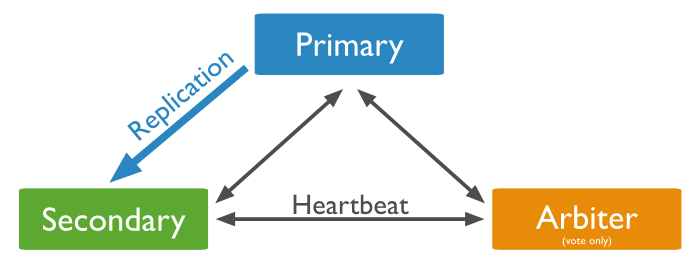
\includegraphics[scale=0.5]{arbiter}
	\caption{Zestaw replik}
\end{figure}

W każdym zestawie replik jeden z węzłów pełni rolę \textit{Primary}. Węzeł ten jest jedynym, który akceptuje operacje zapisu, jest również domyślnym węzłem dla wszystkich operacji odczytu z zestawu replik. Pozostałe węzły wchodzące w skład zestawu, a niebędące węzłem arbitrażowym działają w trybie \textit{Secondary}. Minimalna ilość węzłów zapewniająca poprawną pracę zestawu to 3, ilośc węzłów powinna być nieparzysta.

\begin{figure}[H]
	\centering
		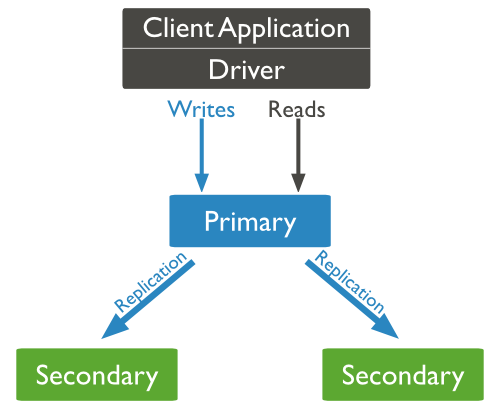
\includegraphics[scale=0.5]{replica-set-read-write-operations-primary}
	\caption{Shemat działania zestawu replik}
	\label{fig:test}
\end{figure}


\subsubsection{Replikacja} 
Replikacja w \textit{MongoDB} jest replikacją asynchroniczą. Węzły \textit{Secondary} replikują dziennik operacji (\textit{oplog}) węzła \textit{Primary} i wykonują operacje w nim zawarte na przechowywanym zbiorze danych.

\subsubsection{Wysoka dostępność}
Zestawe replik gwarantuje wysoką dostępność danych. W przypadku awarii węzła, a w szczególności węzła \textit{Primary}, uruchamiany jest proces \textit{failover}. Ma on na celu zapewnienie płynności dostępu do danych. Pozostałe dziłające węzły w ramach repliki przeprowadzają głosowanie nad wyborem nowego \textit{Primary}, po zakończeniu głosowania zestaw odzyskuje pełną sprawność. Proces \textit{failover} trwa przeważnie poniżej minuty, z czego 10-30 sekund to wykrycie awarii węzła \textit{Primary}, następne 10-30 sekund - proces głosowania. \\
W trakcie głosowania zestaw pracuje w trybie \textit{read-only} - żaden z węzłów nie posiada statusu \textit{Primary} a zatem wszystie żądania zapisu do bazy są odrzucane. \\

\begin{figure}[H]
	\centering
	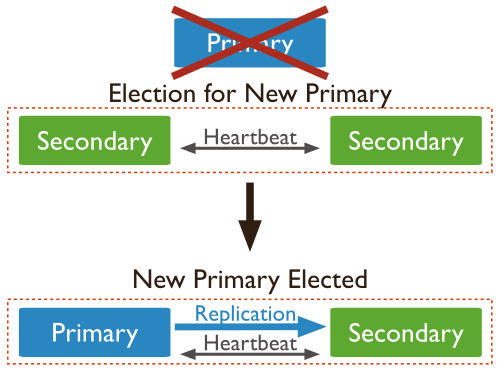
\includegraphics[scale=0.5]{replica-set-trigger-election}
	\caption{Wysoka dostępność z wykorzystaniem procesu \textit{failover}}
\end{figure}

Warunkiem koniecznym do istnienia węzła \textit{Primary} w zestawie, jest dostępność ponad 50\% węzłów. Oznacza to, że dla zestawu składającego się z 3 instancji, jest on w pełni funkcjonalny przy awarii 1 węzła, natomiast zestaw skłądający się z 5 węzłów pozwala na awarię 2 węzłów. \\
W przypadku dostępnośći mniejszej liczby węzłów w zestawie, wszystkie pozostałe przechodzą w tryb \textit{Secondary} - zestaw działa w trybie \textit{read-only}. Mechanizm ten służy zabezpieczeniu danych przed brakiem lub niewystarczającą replikacją w systemie.

\subsubsection{Dostępność}
Poprawne działanie węzłów monitorowane jest za pomocą \textit{Heartbeats}. Instancje co 2 sekundy wzajemnie informują się o poprawnym działaniu, brak informacji przez 10 sekund traktowany jest jako awaria węzłą.

\begin{figure}[H]
	\centering
	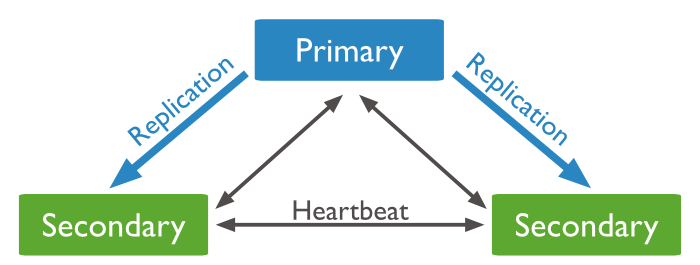
\includegraphics[scale=0.5]{heartbeats}
	\caption{Monitorowanie działania węzłów}
\end{figure}
